\documentclass[fleqn,10pt]{physiome}
% Use option lineno for line numbers 

\articletype{Retrospective}
%% Choose from Original, Retrospective, Review, Letter

\title{Incorporation of sarcolemmal calcium transporters into the Shorten et al. (2007) model of skeletal muscle: equations, coding and stability}

\author[1]{Penelope  J. Noble}
\author[2]{Alan Garny}
\author[3]{Paul R. Shorten}
\author[1]{Kazuyo Tasaki}
\author[2]{Nima Afshar}
\author[1][denis.noble@dpag.ox.ac.uk]{Denis Noble}
\affil[1]{Department of Physiology, Anatomy & Genetics, University of Oxford, United Kingdom}
\affil[2]{Auckland Bioengineering Institute, University of Auckland, New Zealand}
\affil[3]{AgResearch, Ruakura Research Centre, New Zealand}

%% The following lines can be omitted when submitting;
%% information will be added by editors
\publicationdate{28 August 2020}
\editor{Karin Lundengård}
\curator{Anand Rampadarath}
\submitteddate{25 August 2020}
\accepteddate{25 August 2020}
\citethisas{Noble et al. (2020)\\ Incorporation of sarcolemmal calcium transporters into the Shorten et al. (2007) model of skeletal muscle: equations, coding and stability. Physiome.}{10.36903/physiome.12885590}
\begin{document}

\maketitle

\begin{abstract}
We describe a major development of the \citet{shorten2007mathematical} model of skeletal muscle electrophysiology, biochemistry and mechanics. The model was developed by incorporating equations for sarcolemmal transport of calcium ions, including L-type calcium channel, sodium-calcium exchange, calcium pump and background calcium channel. The extended model also includes an addition to the equations for extracellular potassium ion movements to enable the exchange of potassium ions between bulk (plasma) concentration and the interstitial and tubular compartments to be modelled. In further research in an accompanying paper  (Tasaki et al, 2019), we succeeded in reproducing muscle cramp, as well as its prevention and reversal, by investigating muscle contraction and cramp using this extended model in comparison with the original model.
\end{abstract}

\keywords{Skeletal muscle model, L-type calcium channel, sodium-calcium exchange, Ca2+ efflux, potassium}

\primarypubs[10.36903/physiome.12885590]{References}{shorten2007mathematical}

\section{Introduction}

The aim of this paper is to extend the \citet{shorten2007mathematical} skeletal muscle model to include surface membrane calcium transporters. This is necessary to enable the model to be used in applications involving interactions between the surface transporters and either drugs or ions. The extended model was developed specially for a project involving a medication that acts on L-type calcium channels described in an accompanying article (Tasaki et al. 2019).

\section{Model description}

\subsection{Original model}

\begin{figure}[ht!]
\centering
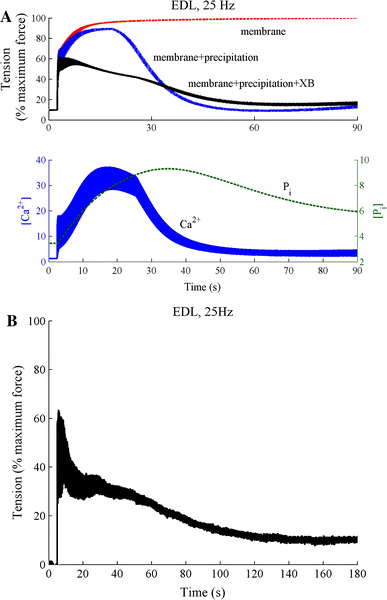
\includegraphics[width=0.5\linewidth]{fig01}
\caption{A - Simulation of force development in the extensor digitorum longus (EDL) fast-twitch version of the model to 90 seconds stimulation at 25 Hz. The curves show the total fatigue response (membrane+precipitation+cross-bridge) along with the responses with no myoplasmic phosphate (Pi) build-up (membrane) and no Pi feedback on the cross-bridge dynamics (membrane+precipitation). Also shown are the calcium and Pi dynamics in a fibre exhibiting total fatigue response (membrane+precipitation+cross-bridge). Once the Pi exceeds a critical threshold it precipitates with SR calcium to reduce calcium release from the SR and cross-bridge cycling kinetics. 
B - the measured EDL response to sustained 25 Hz stimulation. 
(reprinted with permission from \citet{shorten2007mathematical})
}
\label{fig01}
\end{figure}

The skeletal muscle model developed by \citet{shorten2007mathematical} is extensive. It includes models of the action potential, electromechanical coupling, the cross-bridge reactions, and the immediate biochemical processes of consumption of ATP and concentrations of inorganic phosphate. The model was also parameterised to fast and slow twitch fibre types, which have a number of biochemical and biophysical differences. These differences are related to the different force/fatigue responses in fast and slow twitch fibres that are not well understood. A better understanding of the cascade of biochemical and physical events underlying skeletal muscle fatigue will provide a basis for targeted intervention by nutritional or other means to improve muscle function. Loss of muscle function is a major issue in elite athletes, cachectic subjects and those undergoing aging, where muscle function decreases after the age of 40.

The model is available in full working order from the Physiome Model Repository (PMR) at \url{https://models.physiomeproject.org/exposure/487ba7abea1b0ed7ee2ee1bef3f13aee}

Since the model includes the immediate biochemical energetic processes, including variations in ATP and phosphate, it can reproduce the sequence of events underlying muscle fatigue, as shown in \autoref{fig01}. Phosphate is generated during cross-bridge cycling.

\subsection{Explanation why sarcolemmal calcium transporters need to be incorporated}

Electromechanical coupling in smooth and cardiac muscle depends on calcium influx. In both types of muscle, release of calcium ions from the sarcoplasmic reticulum is triggered by calcium-induced calcium release. By this process, a small calcium influx is amplified to produce sufficient calcium to initiate cross-bridge reactions and so produce sliding filament contraction. By contrast, electromechanical coupling in skeletal muscle is purely electrical. Tight coupling between T-tubule membranes through which the action potential propagates makes it possible for SR calcium release to occur even if no calcium influx occurs through the sarcolemmal membrane. Skeletal muscle contractions can therefore continue to occur even in the absence of extracellular calcium. This was demonstrated by \citet{edman1964role}. The immediate effect of exposure of a frog skeletal muscle to nearly zero external calcium was that the muscle continued to contract. Cairns et al. \citep{cairns1998role} found a similar result in mammalian skeletal muscle. Nominally, calcium-free solutions “had little effect on tetanic force in non-fatigued muscle.”

\begin{figure}[ht!]
\centering
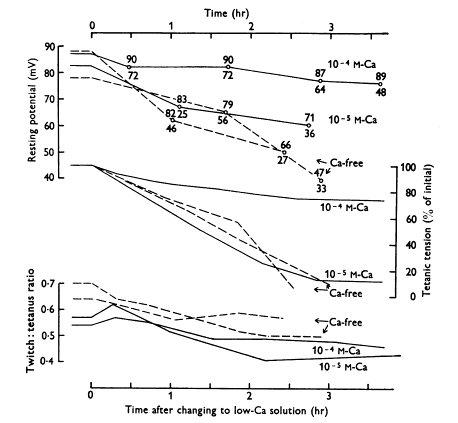
\includegraphics[width=0.7\linewidth]{fig02}
\caption{Effect of lowering calcium concentration in the solution bathing a frog sartorius muscle on mean resting potentials (upper curves; total range of potentials also shown), tetanic tensions (middle curves) and the twitch:tetanus ratio (lower curves). Frog sartorius muscle, temperature 0-1 $^{o}$C. Square pulses of 1 ms duration were applied through two wire electrodes so as to stimulate the whole muscle. Calcium-free solution contained 0.1 mM EDTA. 
(Reprinted with permission from \citet{edman1964role}).
}
\label{fig02}
\end{figure}

However, during prolonged exposure to very low calcium, the twitch contractions fall. In \autoref{fig02}, the muscles were exposed to either 0.1 mM, 0.01 mM calcium or calcium-free Ringer’s solution. Both tetanic tension and the twitch:tetanus ratio slowly declined. This result implies that over long periods of time skeletal muscle does depend on sarcolemmal calcium influx. See Cairns \citep{cairns2003changes,cairns2008multiple} for more discussion on the role of extracellular calcium. 

It is therefore important to incorporate surface membrane calcium fluxes in the \citet{shorten2007mathematical} model. 


\subsection{Methods of incorporating sarcolemmal calcium transporters}

\textbf{L-type calcium current}\newline

The CaV 1.1 and CaV 1.2 L-type calcium channels are found in adult skeletal muscle \citep{jeftinija2007cav, flucher2017and} . CaV 1.1 is restricted to the T-tubules and CaV 1.2 is expressed in the sarcolemma of type I and IIa myofibers, but not IIb fibres.   The data and equations for the L-type calcium current (ICaL) were obtained from the work of \citet{wang2008riluzole} who studied the effect of a sodium channel blocker, Riluzole, on the action potential in cultured human skeletal muscle cells. The equations were taken from the Physiome Model Repository: 

\url{https://models.physiomeproject.org/exposure/3a4c502f78a8c3a5845844b501e153e9}\newline

The equations are:
\begin{equation}
d_{\infty} = \frac{\displaystyle 1}{\displaystyle 1+ e^{\frac{\scriptstyle -24.6-\nu{S}}{\scriptstyle 11.3}}}
\end{equation}

\begin{equation}
\tau_d = \frac{\displaystyle 80\cdot 1}{\displaystyle \cosh -0.031\cdot \left( \nu{S}+37.1 \right)}
\end{equation}

\begin{equation}
\alpha_{d} = \frac{\displaystyle d_{\infty}}{\displaystyle \tau_{d}} 
\end{equation}

\begin{equation}
\beta_{d} = \frac{\displaystyle 1-d_{\infty}}{\displaystyle \tau_{d}} 
\end{equation}

\begin{equation}
\frac{\displaystyle \textrm{d}d}{\displaystyle \textrm{d}time} = \alpha_{d}\cdot \left( 1-d \right) -\beta_{d}\cdot d
\end{equation}

\begin{equation}
f_{\inf} = \frac{1}{1+e^\frac{\nu{S}+S}{7}}
\end{equation}

\begin{equation}
I_{Ca} = g_{Ca}\cdot d^{\scriptstyle 2}\cdot f_{inf}\cdot \left( \nu{S}-E_{Ca} \right)     
\end{equation}

The equation for the inactivation (f$_{inf}$) process was added for use in a future project.\newline 

\textbf{Sodium-calcium exchange}\newline

The data and equations for sodium-calcium exchange (NCX) were obtained from \citet{noble1991role}, which were originally developed by \citet{di1985model} and which reproduce the data obtained by \citet{kimura1987identification} for cardiac muscle. NCX is based on 3:1 stoichiometry \citep{michel2014function}. NCX is also more abundant in slow twitch fibres, which is consistent with a role for NCX in fatigue resistance \citep{michel2014function}.\newline

The equation is:\newline

\begin{equation}
    I_{NaCa} = \frac{k_{NaCa}.(\exp{\frac{\gamma.(n_{NaCa}-2).\nu_{s}.FF}{RR.TT}}.Na_i^{n}.Ca_{0}-\frac{\exp{\frac{(\gamma-1).(n_{NaCa}-2).\nu_{s}.FF}{RR.TT}}.Na_i^{n}.Ca_{2}}{1000})}{(1+d_{NaCa}.(\frac{Ca_2}{1000}.Na_e^n+Ca_0.Na_i^n)).(1+\frac{Ca_2}{1000\times0.0069})}
\end{equation}

\textbf{Calcium pump}\newline

The data and equations for the calcium pump current, IpCa, were obtained from
\citet{lindblad1996model} in cardiac muscle.\newline
The equation is:\newline

\begin{equation}
    I_{pCa} = \frac{\frac{i_{CaPmax}.Ca_2}{1000}}{\frac{Ca_2}{1000}+k_{CaP}}
\end{equation}

\textbf{Background calcium leak}\newline

The data and equations for the background calcium current leak, IbCa, were obtained from \citet{noble1991role}.\newline

The equation is: \newline

\begin{equation}
    I_{bCa} = g_{bca}.(\nu_S - E_{Ca})
\end{equation}

g$_{bCa}$ was usually set to zero. The calcium pump and sodium-calcium exchange were sufficient to balance calcium movements in steady state conditions. 

To represent the bulk potassium concentration outside the muscle, [K]b (which is equivalent to a plasma potassium concentration), we added a term to the differential equation for interstitial potassium, K$_e$, which then becomes:

\begin{equation}
    \frac{\partial K_e}{\partial time} = 1. (\frac{I_{IR}+I_{DR}+I_{{K}_{rest}}+ - 2.I_{NaK}}{\frac{1000}{1}.FF.tsi3}+\frac{K_t-K_e}{\tau_{k2}}+\frac{K_b-K_e}{\tau_{k3}})
\end{equation}

[K]$_b$ is assumed to be fixed.\newline

The original CellML file along with all the codes can be found in the following link in the PMR:\newline

\url{https://models.physiomeproject.org/workspace/5c6}

It is worth to mention that in order to be able to run python scripts the corresponding sedml and cellml files need to be downloaded in the same folder. Also In order to be able to run sedml file the corresponding cellml file needs to be downloaded in the same folder.


\section{Model results}

All simulations were run using OpenCOR (version 0.6) \citep{garny2015opencor}\newline(\url{http://opencor.ws})\newline

\textbf{Comparison with the original model over short pulse trains}\newline

\begin{figure}[ht]
\centering
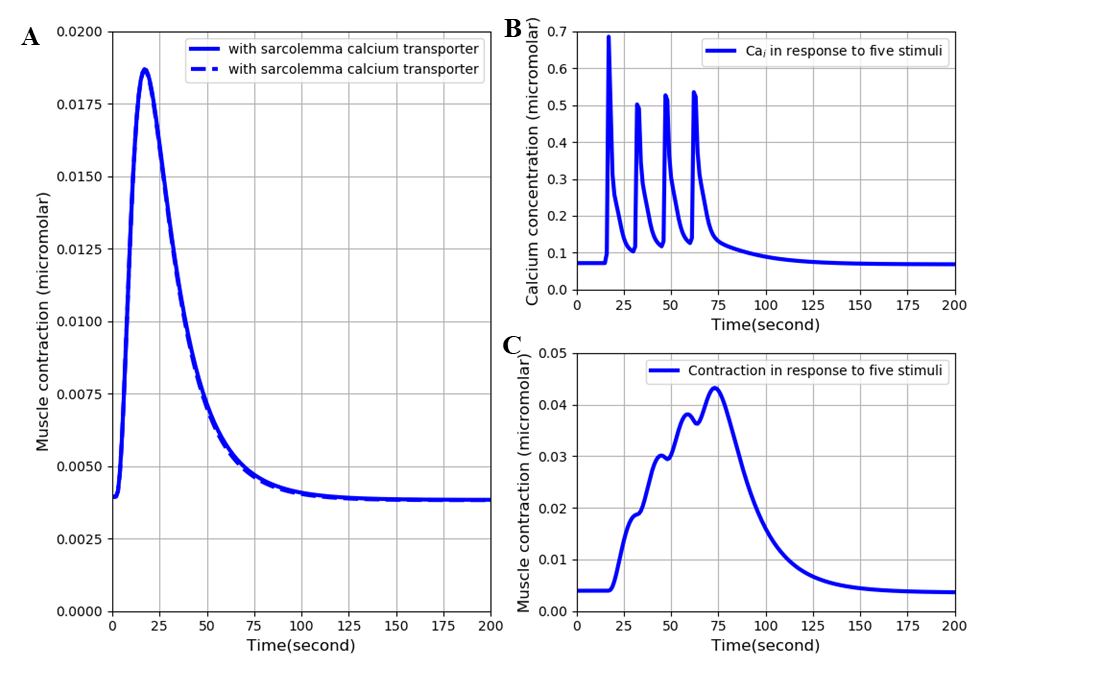
\includegraphics[width=1\linewidth]{fig03.png}
\caption{A: superimposed contraction responses to a single stimulus with and without (lighter curve) the surface calcium transporters. B: free intracellular calcium and C: contraction in response to a train of five stimuli at 15-second intervals. The results are similar to those of Figures 6 and 11 in the original \citet{shorten2007mathematical} model. The results presented in the left panel can be reproduced with the \href{https://models.physiomeproject.org/workspace/5c6/file/afd4d5cb20ecdcbc0b10198fe31795520488a34e/Fig03(L).py}{Fig03(L).py} script in OpenCOR and those in the right panel with \href{https://models.physiomeproject.org/workspace/5c6/file/afd4d5cb20ecdcbc0b10198fe31795520488a34e/Fig03(R).py}{Fig03(R).py}}
\label{fig03}
\end{figure}


\autoref{fig03} shows the results of calculating the free intracellular calcium and contraction following a single pulse and a short train of 5 stimuli with and without the surface calcium transporters. The simulation files \href{https://models.physiomeproject.org/workspace/5c6/file/afd4d5cb20ecdcbc0b10198fe31795520488a34e/Fig03(L).sedml}{Fig03(L).sedml} and \href{https://models.physiomeproject.org/workspace/5c6/file/afd4d5cb20ecdcbc0b10198fe31795520488a34e/Fig03(R).sedml}{Fig03(R).sedml} contain the computational setting for running the model with a single pulse and 5 stimuli respectively.
% To obtain the plots of simulation results, use the python code for figure \ref{fig03} in the supplementary material.

The difference between the results with and without the surface calcium transporters is very small. Adding those transporters does not therefore significantly affect the behaviour of the model over short time periods. This result would be expected since the surface calcium fluxes are very small and do not have much impact on intracellular ion concentrations when short durations are considered.

The curves also compare well qualitatively with Figures 6 and 11 in the original model paper. There is, however, an important quantitative difference arising from the fact that we used initial conditions obtained from running the extended model for very long periods (hours) to achieve steady state conditions. With the original model parameters, this produces a lower initial state of intracellular calcium and, therefore, much lower contraction than in the \citet{shorten2007mathematical}. paper. 

We also ran these computations using the initial conditions, i.e. not steady state conditions, obtained from the CellML file for the original model on PMR. These results were very similar qualitatively to those shown in \autoref{fig03}, except that the contraction was much larger. There was nevertheless still a difference from the published \citet{shorten2007mathematical} paper. The contraction was found to be about 50\% of that in the original paper.

\textbf{Test of calcium balance}\newline

Although the equations for influx of calcium through ICaL were obtained on skeletal muscle, the equations for efflux of calcium via sodium-calcium exchange and the calcium pump were obtained from heart muscle models. NCX1 is expressed in high levels in cardiac muscle. NCX1 is also found in skeletal muscle \citep{cifuentes2000sodium}, where it is found in sarcolemma and T-tubule membranes \citep{sacchetto1996colocalization}. The major function of the skeletal muscle NCX appears to be to transport calcium out of the cell after contraction.\newline

Their role in the model is to balance the influx and efflux so that over many cycles of normal physiological muscle activity there would be no net change in calcium content of the muscle fibres. We adjusted their amplitudes until balance was achieved, as shown in \autoref{fig04}. The simulation file \href{https://models.physiomeproject.org/workspace/5c6/file/afd4d5cb20ecdcbc0b10198fe31795520488a34e/Fig04.sedml}{Fig04.sedml} contains the computational setting for running the model.

\begin{figure}[ht]
\centering
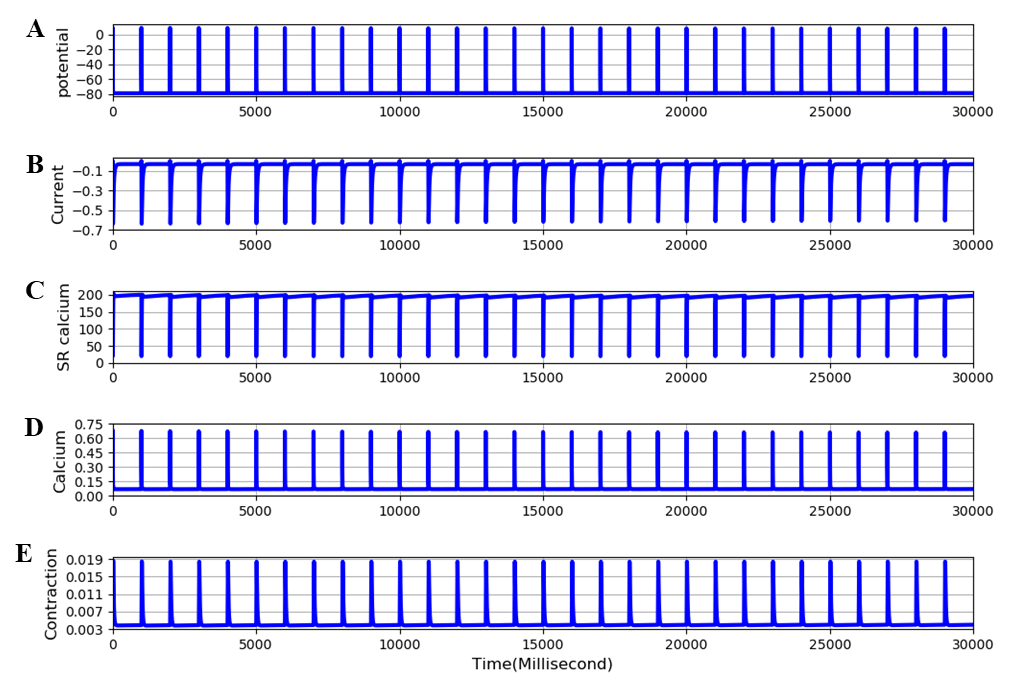
\includegraphics[width=1\linewidth]{fig04}
\caption{Extended EDL model. Traces are: A - membrane potential, B - calcium current, C - SR calcium, D - free intracellular calcium, E - twitch contraction. The frequency of stimulation is 1 Hz. All parameters are in steady state conditions over 30 cycles of stimulation. The results presented in this figure can be reproduced with the \href{https://models.physiomeproject.org/workspace/5c6/rawfile/afd4d5cb20ecdcbc0b10198fe31795520488a34e/Fig04.sedml}{Fig04.sedml}} 
\label{fig04}
\end{figure}

\textbf{Effect of blocking calcium influx}

\begin{figure}[ht]
\centering
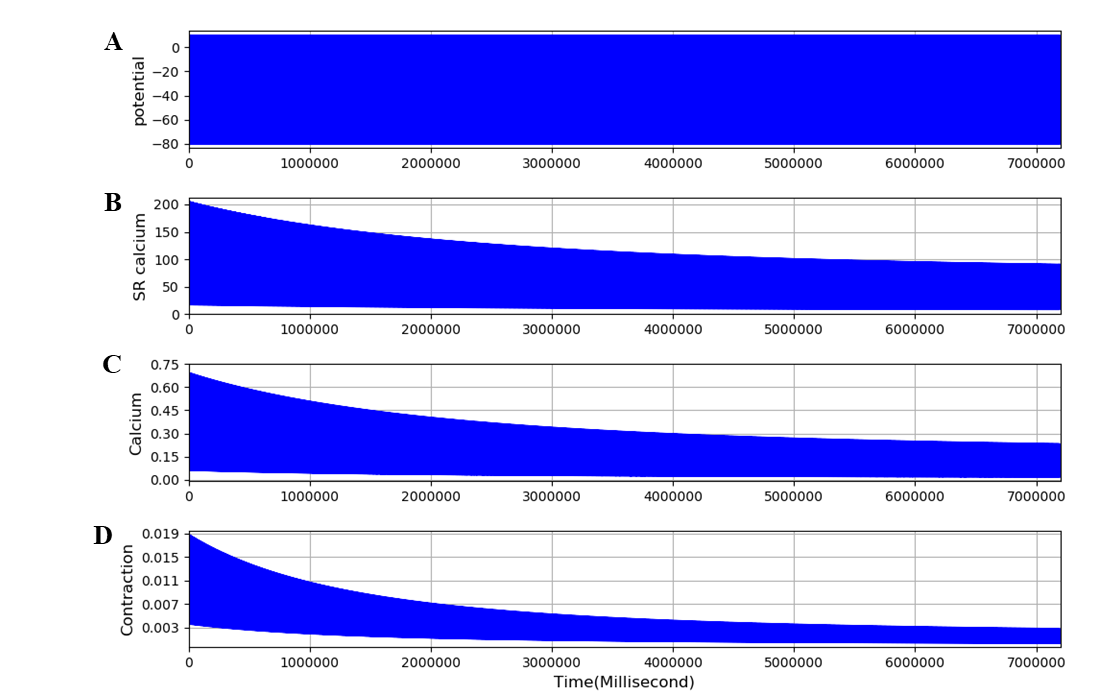
\includegraphics[width=0.9\linewidth]{fig05}
\caption{Extended model run for 2 hours with the L-type calcium channel completely blocked. Traces are: A - membrane potential, B - calcium current, C - SR calcium, D - free intracellular calcium, E - twitch contraction. The frequency of stimulation is 0.1 Hz. The results presented in this figure can be reproduced with the \href{https://models.physiomeproject.org/workspace/5c6/file/afd4d5cb20ecdcbc0b10198fe31795520488a34e/Fig05.sedml}{Fig05.sedml}} 
\label{fig05}
\end{figure}

\autoref{fig05} shows that, when the L-type calcium channel is blocked, the model is no longer in a steady state. SR calcium, free intracellular calcium and contraction all decline slowly, as observed by \citet{edman1964role} in their experiments in skeletal muscle in low or zero external calcium. The model achieves a new steady state after 1-2 hours. This very slow change and its experimental validation is dealt with in a further paper (Tasaki et al., 2019). The simulation file \href{https://models.physiomeproject.org/workspace/5c6/file/afd4d5cb20ecdcbc0b10198fe31795520488a34e/Fig05.sedml}{Fig05.sedml} contains the computational setting for running the model.
In addition to incorporating equations for surface membrane calcium fluxes, we added a term to the extracellular potassium equations to represent the movement of potassium ions between extracellular spaces (interstitial and tubular) within the muscle structure and the spaces outside the muscle, which would include blood plasma potassium. This feature of the extended model is used in an accompanying paper (Tasaki et al., 2019) to model the effects of potassium wash-out during increased blood flow. \autoref{fig06} shows that the equations behave as expected. The bulk (plasma) potassium, [K]b, was switched suddenly between 5 and 2 mM twice during the calculation. The time constant, TauK3, was arbitrarily set to 4 seconds to represent fast perfusion of the interstitial space. Interstitial potassium correctly follows an exponential decline when [K]b is switched to 2 mM and recovers equally rapidly when [K]b is returned to 5mM. The use of this process in representing perfusion of the interstitial space is shown in the accompanying paper (Tasaki et al., 2019). The simulation file \href{https://models.physiomeproject.org/workspace/5c6/file/afd4d5cb20ecdcbc0b10198fe31795520488a34e/Fig06.sedml}{Fig06.sedml} contains the computational setting for running the model.\newline

\begin{figure}[ht]
\centering
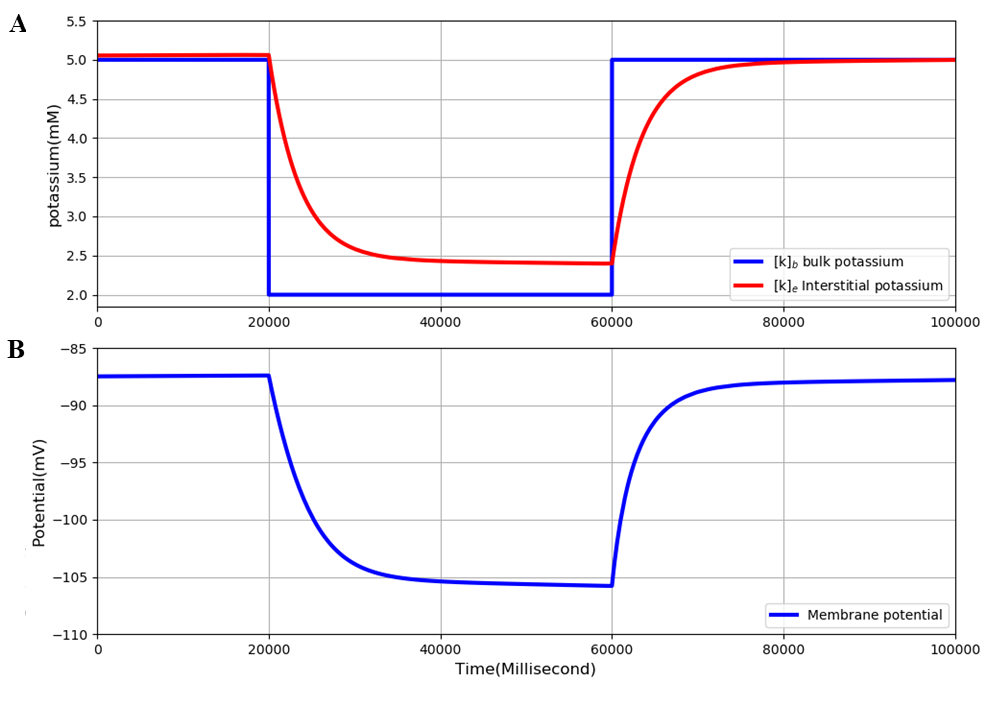
\includegraphics[width=0.9\linewidth]{fig06}
\caption{Extended model run for 10 minutes. [K]b was initially set at 5 mM and then switched to 2 mM and later returned to 5 mM. A - Interstitial potassium correctly responds to these changes. B - The membrane potential also responds correctly. The results presented in \autoref{fig06} can be reproduced with the \href{https://models.physiomeproject.org/workspace/5c6/file/afd4d5cb20ecdcbc0b10198fe31795520488a34e/Fig06.py}{Fig06.py} script in OpenCOR} 
\label{fig06}
\end{figure}

\textbf{Deficiency of the extended model}\newline

As already noted, when the results shown in Figures \ref{fig04} and \ref{fig05} are examined carefully, the magnitude of the contractions is clearly very much smaller than in the original \citet{shorten2007mathematical} model. The computed steady state cross-bridge reactions are much less than 1 µM, whereas in the original model the reactions are at least an order of magnitude larger.  The reason for this discrepancy is that the model was not parameterised for very long runs, of hours rather than minutes. All our computations are performed when the extended model has achieved steady state after about 2 hours since we need a steady state condition to study the dynamics of change from the steady state when the model is perturbed, e.g. by partial or complete block of the L-type calcium channel, as done in the accompanying paper (Tasaki et al., 2019).

We therefore investigated whether a simple parameter change could restore the magnitude of steady state contraction after very long time periods. Since the low value of calcium and contraction after 2 hours represents a loss of sarcoplasmic reticulum calcium, we investigated the effect of increasing the uptake rate for calcium entry into the SR, nuSR. \autoref{fig07} shows that this simple parameter change can indeed increase the steady state contraction by more than an order of magnitude. When nuSR is increased to 35 the contraction increases from around 0.02 to 0.8. The simulation file \href{https://models.physiomeproject.org/workspace/5c6/file/afd4d5cb20ecdcbc0b10198fe31795520488a34e/Fig07.sedml}{Fig07.sedml} contains the computational setting for running the model for only one value of nuSR. Peak value of contraction was plotted versus different nuSR (5, 15, 25, 35).\newline

\begin{figure}[h!]
\centering
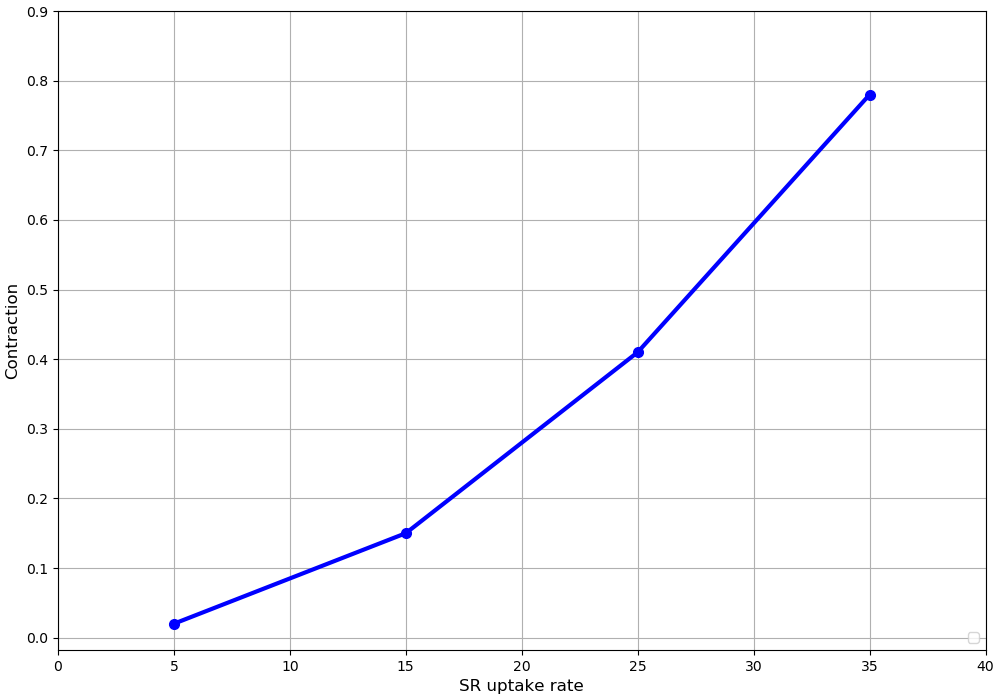
\includegraphics[width=0.8\linewidth]{fig07}
\caption{Computed relation between the SR uptake rate, nuSR, and the steady state contraction at a frequency of stimulation of 0.1 Hz. The standard value of nuSR, 4.875, allows the SR to empty over long periods so that the cross-bridge activation by released calcium is very small. Increasing nuSR to 15, 35 and 45 5produces much larger contractions. The results presented in \autoref{fig07} can be reproduced with the \href{https://models.physiomeproject.org/workspace/5c6/file/afd4d5cb20ecdcbc0b10198fe31795520488a34e/Fig07.py}{Fig07.py} and \href{https://models.physiomeproject.org/workspace/5c6/file/afd4d5cb20ecdcbc0b10198fe31795520488a34e/Fig07-plot.py}{Fig07-plot.py} script in OpenCOR} 
\label{fig07}
\end{figure}

However, the results also showed that further increase of nuSR (e.g to 45) prevented the membrane potential from fully repolarizing. The reason is that the increased calcium release during each contraction activates the sodium-calcium exchange, so producing a larger after-potential. 

There is therefore a deficiency that requires further re-parameterisation of the extended model in future applications.\newline

\section{Discussion}


Sarcolemmal calcium influx is not necessary for individual twitch responses in skeletal muscle since the membrane trigger for electromechanical coupling is entirely electrical, independent of calcium current. This property is what enabled \citet{shorten2007mathematical} to reproduce fatigue in their model with only intracellular recycling of calcium.\newline

However, by adding equations for the sarcolemmal calcium fluxes we have shown that over periods of time greater than a few seconds, the sarcolemmal calcium fluxes would be expected to have a significant effect.  Specifically, the small fluxes gradually alter SR calcium and intracellular free calcium. These changes in calcium concentrations then produce changes in contraction. The slow time course of those changes corresponds to the dynamics of change in contraction observed experimentally when calcium influx is reduced, as shown in the accompanying paper (Tasaki et al., 2019). The influences of changes in sodium, potassium and calcium ion concentrations, on the contraction of skeletal muscle are very complex \citep{cairns1998role, cairns2003changes, cairns2008multiple}. Future work on the extended model needs to be done to determine the extent to which the model could help to clarify these effects. \newline

Further work also needs to be done to explore parameter sets that would increase the steady state contraction to be comparable to the contraction level calculated in the original model. A possible way forward to be developed in the future would be to rebalance the proportion of calcium efflux attributable to sodium-calcium exchange compared to the sarcolemmal calcium pump. The sodium-calcium exchange produces a depolarizing current, whereas the calcium pump does not do so. We have not systematically explored this question in this paper since it is likely that other parameter adjustments may also be required. The parameter space to be explored may be quite large.

\section{Acknowledgements}
We express our gratitude to TSUMURA & CO. for funding the “University of Oxford Innovative Systems Biology Project sponsored by Tsumura”. 

\bibliography{References}
\end{document}